\chapter{Arquitetura de \textit{Hardware}  (RTL)}
\section{Gerenciamento de Processamento: Módulo \texttt{cnn\_top}}

O processamento da CNN é gerenciado por um módulo superior (\texttt{cnn\_top}), que instancia 9 submódulos responsáveis pela inferência da rede, coordenando-os por meio de uma Máquina de Estados Finitos (FSM) própria.

Além dos sinais oriundos dos submódulos instanciados e dos sinais básicos de \textit{clock} e \textit{reset}, o \texttt{cnn\_top} recebe três sinais externos. Dois deles vêm da lógica do controlador VGA e são utilizados na leitura do \textit{framebuffer}. O terceiro é o \textit{\textit{bit}} recebido pela comunicação serial, que passa por dois \textit{flip-flops} para mitigar problemas de metaestabilidade antes de ser enviado ao módulo UART.

As principais saídas do \texttt{cnn\_top} usadas pelo arquivo principal do projeto são detalhadas na Tabela \ref{tab:sinais_cnn_top}.

\begin{table}[htbp]
\centering
\caption{Principais saídas do módulo \texttt{cnn\_top}}
\label{tab:sinais_cnn_top}
\small
\begin{tabularx}{\textwidth}{l X}
\toprule
\textbf{Sinal} & \textbf{Descrição} \\
\midrule
\texttt{class\_id[4:0]} & Valor da classe predita (0 = Vazio, 1 = Desconhecido, 2 a 19 = Autorizados). \\
\texttt{access\_done} & Sinal que indica a finalização do processo de inferência. \\
\texttt{frame\_ready} & Sinal ativo quando o \textit{framebuffer} $32 \times 32$ está completo. \\
\texttt{frame\_mode} & Indica se a exibição será o vídeo completo ou apenas o recorte do rosto. \\
\bottomrule
\end{tabularx}
\end{table}

% TODO: Inserir diagrama das principais entradas e saídas do bloco cnn_top
\begin{figure}[H]
    \centering
    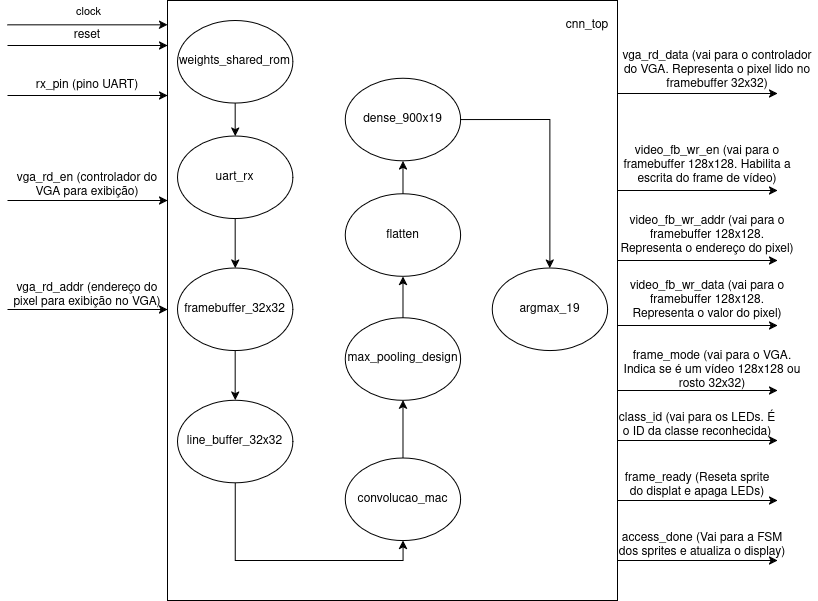
\includegraphics[width=0.7\textwidth]{imagens/image18.png}
    \caption{Diagrama de blocos das principais entradas e saídas do módulo \texttt{cnn\_top}.}
    \label{fig:diagrama_cnn_top}
\end{figure}

\subsection{Papel e Comportamento dos Submódulos}

O papel e o comportamento de cada submódulo instanciado são detalhados a seguir:

\subsubsection{UART}
Responsável pela decodificação da comunicação serial em \textit{bytes} de 8 \textit{bits}.

\begin{table}[htbp]
\centering
\caption{Principais sinais do submódulo UART}
\label{tab:sinais_uart}
\small
\begin{tabularx}{\textwidth}{l X}
\toprule
\textbf{Sinal} & \textbf{Descrição} \\
\midrule
\texttt{data\_out[7:0]} & O \textit{byte} completo montado após a recepção serial. \\
\texttt{data\_valid} & Pulso indicando que \texttt{data\_out} contém um \textit{byte} válido. \\
\bottomrule
\end{tabularx}
\end{table}

\subsubsection{\textit{Framebuffer} $32 \times 32$}
Responsável pela escrita espelhada em duas memórias internas distintas de 1024 \textit{bytes}, permitindo a leitura simultânea pela CNN e pelo módulo VGA em frequências diferentes. Durante a escrita, recebe sinais de controle e de endereço do \texttt{cnn\_top}, processando os dados advindos da UART. Na leitura da rede, a FSM do \texttt{cnn\_top} envia sinais de requisição e recebe o pixel correspondente. Para a exibição em tela, o controlador VGA faz requisições similares na segunda memória. Ao receber um sinal de \textit{reset}, todos os endereços de ambas as memórias são zerados (\texttt{0x00}).
\begin{table}[htbp]
\centering
\caption{Principais sinais do submódulo \textit{Framebuffer} $32 \times 32$}
\label{tab:sinais_framebuffer}
\small
\begin{tabularx}{\textwidth}{l X}
\toprule
\textbf{Sinal} & \textbf{Descrição} \\
\midrule
\texttt{rd\_data[7:0]} & \textit{Byte} que representa o pixel solicitado pela CNN durante a leitura do \textit{framebuffer}. \\
\texttt{frame\_ready} & Pulso que indica quando o último pixel foi armazenado durante a escrita. \\
\texttt{vga\_rd\_data[7:0]} & \textit{Byte} que representa o pixel solicitado pelo VGA durante a leitura do \textit{framebuffer}. \\
\bottomrule
\end{tabularx}
\end{table}

\subsubsection{\textit{Line Buffer}}
Durante a leitura da imagem, o módulo de \textit{Line Buffer} produz e armazena a janela $3 \times 3$ a partir do fluxo sequencial de pixels, fornecendo a matriz necessária para a convolução. Como a leitura ocorre da esquerda para a direita e de cima para baixo, o módulo retém o histórico das duas últimas linhas da imagem em blocos de memória dedicados. O deslocamento espacial para formar a janela é coordenado por sinais de controle. Ao associá-las ao pixel atual de entrada, consegue formar a saída desejada.

\begin{table}[htbp]
\centering
\caption{Principais sinais do submódulo \textit{Line Buffer}}
\label{tab:sinais_linebuffer}
\small
\begin{tabularx}{\textwidth}{l X}
\toprule
\textbf{Sinal} & \textbf{Descrição} \\
\midrule
\texttt{win[0:8][7:0]} & A ``janela'' $3 \times 3$ completa formada por cada pixel. \\
\texttt{window\_valid} & Pulso que indica a finalização da construção de uma janela válida. \\
\bottomrule
\end{tabularx}
\end{table}

\subsubsection{Convolução}
Executa a convolução 2D sobre a janela $3 \times 3$ gerada pelo \textit{Line Buffer}. Recebe os pesos e vieses dos 4 filtros quantizados em ponto fixo Q1.7. Para cada filtro, a operação de multiplicação e acumulação (MAC) segue a formulação matemática:

$$ MAC = \sum_{i} pixel(i) \cdot peso(i) + bias, \text{onde } i \in \{0, \dots, 8\} $$

Para evitar \textit{overflow} de informações, os acumuladores são operados em 20 \textit{bits} (quantizados em Q6.14). Em seguida, aplica-se a função de retificação linear (ReLU), na qual valores negativos são descartados (zerados) e valores superiores a 32767 são saturados. O resultado é truncado para 16 \textit{bits} no formato Q2.14. A cada ciclo de \textit{clock}, ele produz 4 saídas (uma por filtro):

\begin{table}[htbp]
\centering
\caption{Principais sinais do submódulo de Convolução}
\label{tab:sinais_convolucao}
\small
\begin{tabularx}{\textwidth}{l X}
\toprule
\textbf{Sinal} & \textbf{Descrição} \\
\midrule
\texttt{out\_f0} & Pixel resultante da convolução da janela com o filtro 0. \\
\texttt{out\_f1} & Pixel resultante da convolução da janela com o filtro 1. \\
\texttt{out\_f2} & Pixel resultante da convolução da janela com o filtro 2. \\
\texttt{out\_f3} & Pixel resultante da convolução da janela com o filtro 3. \\
\texttt{valid\_out} & Pulso que valida a saída da convolução. \\
\bottomrule
\end{tabularx}
\end{table}

\subsubsection{\textit{Max \textit{Pooling} }}
Possui quatro memórias para armazenar a linha anterior processada pelos 4 filtros. Por meio de um circuito combinacional, compara os quatro valores de cada sub-janela $2 \times 2$ espacial, repassando apenas o valor máximo. O módulo opera com um \textit{stride} de 2, calculando janelas apenas em coordenadas ímpares. Como gera 4 resultados simultâneos e o próximo estágio consome apenas 1 por ciclo, implementa-se um sistema FIFO de 32 posições para serializar as saídas.

\subsubsection{\textit{Flatten}  (``Achatamento'')}
Como a convolução aplicada não possui \textit{padding valid}, a imagem original $32 \times 32$ é reduzida para $30 \times 30$. Após o \textit{Pooling}, a dimensionalidade cai para $15 \times 15$ por filtro. Este módulo funciona essencialmente como um contador, serializando cada pixel recebido até atingir os 900 valores esperados ($15 \times 15 \times 4$).

\subsubsection{Camada Densa}
Responsável por realizar a classificação final. O módulo recebe cada pixel proveniente do \textit{Flatten}  e realiza o cálculo MAC com 19 pesos simultâneos (um para cada classe), acumulando os resultados ao longo dos ciclos de \textit{clock}. Quando os 900 pixels são finalizados, a camada soma os vieses. Utilizam-se acumuladores de 48 \textit{bits} para reter precisão.

\begin{table}[H]
\centering
\caption{Principais sinais do submódulo de Camada Densa}
\label{tab:sinais_camada_densa}
\small
\begin{tabularx}{\textwidth}{l X}
\toprule
\textbf{Sinal} & \textbf{Descrição} \\
\midrule
\texttt{valid\_out} & Pulso de controle que informa para o módulo seguinte que o processamento da camada densa foi concluído. \\
\texttt{done} & Pulso de controle que informa para o \texttt{cnn\_top} que o processamento da camada densa se encerrou. \\
\texttt{scores[0:18][15:0]} & 19 valores de 16 \textit{bits} formatados em Q6.10 que serão usados pelo módulo final para a inferência. \\
\bottomrule
\end{tabularx}
\end{table}

\subsubsection{Argmax}
Módulo que executa o processo final de decisão. Opera como uma FSM que varre as saídas da Camada Densa comparando os \textit{scores}. A classe correspondente ao maior valor é definida como a predição da rede. O índice gerado é internamente incrementado em 1 para se adequar à lógica do VGA, que reserva o ID 0 para a tela vazia (isto é, sem qualquer exibição de nomes).

\begin{table}[H]
\centering
\caption{Principais sinais do submódulo Argmax}
\label{tab:sinais_argmax}
\small
\begin{tabularx}{\textwidth}{l X}
\toprule
\textbf{Sinal} & \textbf{Descrição} \\
\midrule
\texttt{valid\_out} & Pulso de controle para indicar a finalização da inferência. \\
\texttt{class\_id[4:0]} & ID da classe inferida. \\
\bottomrule
\end{tabularx}
\end{table}

\subsubsection{ROM de Pesos}
Módulo responsável por ler o arquivo \texttt{.mif} de inicialização e rotear os parâmetros da rede. Ele transfere os pesos para registradores (no caso das camadas iniciais) ou blocos M9K (no caso da camada densa). Para permitir o acesso paralelo aos 19 pesos da camada densa em um único ciclo, estes são distribuídos em 19 blocos M9K individuais. Além dos parâmetros de cada camada, sua saída também inclui um \textit{bit} de controle indicando a conclusão das cópias de cada endereço.

\newpage
\noindent \textbf{Observações Importantes:}
\begin{itemize}
    \item As saídas dos módulos de \textit{Max \textit{Pooling}}  e \textit{Flatten}  são somente os pulsos de controle e o dado processado naquele bloco.
    \item A camada densa não aplica quaisquer funções de ativação. Isso ocorre por conta da lógica de escolha da saída da rede: a previsão é o ID, isto é, a posição do maior valor calculado. Importante também observar que a classe ``Desconhecido'' foi tratada como uma classe real, em contraposição à interpretação desta como a negação de todas as demais.
\end{itemize}

\subsection{Máquina de Estados de Controle}

Conhecendo os principais sinais que o \texttt{cnn\_top} gerencia, é possível descrever a FSM que controla a CNN conforme o diagrama da Figura \ref{fig:fsm_cnn} e a Tabela \ref{tab:sinais_cnn_top}.

% TODO: Inserir diagrama da FSM
\begin{figure}[H]
    \centering
    \includegraphics[width=1\textwidth]{imagens/image13.png}
    \caption{Diagrama de estados da FSM controladora da CNN no módulo \texttt{cnn\_top}.}
    \label{fig:fsm_cnn}
\end{figure}

\begin{table}[H]
\centering
\caption{Sinais de controle da FSM principal do módulo \texttt{cnn\_top}}
\label{tab:sinais_fsm_controle}
\small
\begin{tabularx}{\textwidth}{l X}
\toprule
\textbf{Sinal} & \textbf{Descrição} \\
\midrule
\texttt{argmax\_valid} & Conexão no \texttt{cnn\_top} que recebe a saída \texttt{valid\_out} do módulo Argmax. \\
\texttt{uart\_valid} & Conexão no \texttt{cnn\_top} que recebe a saída \texttt{data\_valid} do módulo UART. \\
\texttt{uart\_data} & Conexão no \texttt{cnn\_top} que recebe a saída \texttt{data\_out} do módulo UART. \\
\texttt{uart\_wr\_addr} & Sinal gerado pelo módulo \texttt{cnn\_top} durante a leitura do \textit{framebuffer}. É um contador que incrementa a cada novo \textit{byte} recebido. \\
\texttt{uart\_frame\_pending} & Sinal de controle. Enquanto a imagem está sendo lida, é 0. Sobe para 1 apenas quando \texttt{uart\_wr\_addr == 1023}. \\
\texttt{frame\_ready} & Conexão no \texttt{cnn\_top} que recebe a saída \texttt{frame\_ready} do \textit{framebuffer}. \\
\texttt{frame\_mode} & Pulso de saída que indica ao VGA se a exibição deverá ser de um rosto ou do vídeo. \\
\texttt{weights\_boot\_done} & Sinal de controle que indica que o processo de gravação de pesos foi concluído. \\
\texttt{frame\_clear} & Sinal enviado para ``desligar'' o \texttt{frame\_ready} assim que a rede inicia uma nova inferência. \\
\texttt{rd\_val\_count} & Contador que indica o progresso de leitura da memória síncrona M9K. \\
\bottomrule
\end{tabularx}
\end{table}

\section{Validação da Arquitetura de \textit{Hardware} }

Para validar as inferências em ponto fixo realizadas pelo \textit{hardware}, fez-se necessária a comparação dessas saídas com seus respectivos valores em ponto flutuante, obtidos via \textit{software}. Para tanto, considerando uma mesma imagem de entrada, adotaram-se procedimentos e métricas específicas de avaliação, estruturados da seguinte forma:

\begin{enumerate}
    \item \textbf{Seleção das Camadas:} Os valores comparados correspondem às saídas dos módulos de Convolução, \textit{Max \textit{Pooling}}, \textit{Flatten}, Camada Densa e ao resultado final da inferência.
    \item \textbf{Extração e Quantização em Software:} Cada valor foi extraído do modelo em \textit{software} e quantizado para o formato de ponto fixo equivalente ao do \textit{hardware}. Nas camadas de convolução, \textit{Pooling} e \textit{Flatten}, os valores foram multiplicados por $2^{14}$ e arredondados. Na camada densa, a saída foi calculada sem a aplicação da função de ativação (\textit{Softmax}) e, em seguida, quantizada no formato Q6.10.
    \item \textbf{Extração em \textit{Hardware} :} Os valores processados fisicamente pelo circuito foram capturados por meio de um \textit{testbench} específico escrito em Verilog.
    \item \textbf{Estruturação dos Dados:} Ao final das extrações, geraram-se pares de arquivos \texttt{.txt} (um contendo as saídas do \textit{software} e outro as do \textit{hardware}) com a mesma estrutura de organização e quantização para cada camada analisada.
\end{enumerate}

De posse de cinco arquivos de \textit{log} para cada ambiente de execução, as seguintes métricas foram calculadas:
\subsection{Métricas de Avaliação}

\noindent\textbf{Erro Absoluto Médio (MAE):} Representa a soma das diferenças, em módulo, calculada ponto a ponto e dividido pelo número total de pontos. Expressa a distância absoluta média entre a saída teórica e a saída física.
\begin{equation}
\text{MAE} = \frac{1}{N} \sum_{i=1}^{N} \left| \text{HW}_i - \text{SW}_i \right|
\end{equation}
Onde $N$ é o número total de amostras da camada, $\text{HW}$ é o valor computado no \textit{hardware} e $\text{SW}$ é o valor extraído no \textit{software}.

\noindent\textbf{Raiz do Erro Quadrático Médio (RMSE):} Avalia a magnitude do erro, penalizando desvios maiores. Caso não ocorram valores excessivamente discrepantes (\textit{outliers} decorrentes de \textit{overflow}), espera-se que o RMSE permaneça próximo ao MAE.
\begin{equation}
\text{RMSE} = \sqrt{\frac{1}{N} \sum_{i=1}^{N} \left( \text{HW}_i - \text{SW}_i \right)^2}
\end{equation}

\noindent\textbf{Erro Máximo Absoluto (MaxErr):} Serve para identificar o desvio do pior cenário dentro da execução de uma camada.
\begin{equation}
\text{MaxErr} = \max_{i=1}^{N} \left| \text{HW}_i - \text{SW}_i \right|
\end{equation}

\noindent\textbf{Percentual de Valores Exatos (\%):} Mede a taxa de acerto onde houve paridade perfeita entre os valores.
\begin{equation}
\mathrm{Exatid\~ao} =
\frac{1}{N}
\sum_{i=1}^{N}
\mathds{1}\!\left[HW_i = SW_i\right]
\times 100,
\end{equation}
Onde $\mathds{1}[\cdot]$ é a função indicadora, assumindo valor $1$ quando a condição é verdadeira e $0$ caso contrário.

\noindent\textbf{Coeficiente de Correlação de \textit{Pearson} ($r$):} Mede o grau de correlação linear e a proporcionalidade entre as duas distribuições de saída.
\begin{equation}
r =
\frac{
\sum_{i=1}^{N}
\left(\mathrm{SW}_i-\overline{\mathrm{SW}}\right)
\left(\mathrm{HW}_i-\overline{\mathrm{HW}}\right)
}{
\sqrt{
\sum_{i=1}^{N}\left(\mathrm{SW}_i-\overline{\mathrm{SW}}\right)^2
\;
\sum_{i=1}^{N}\left(\mathrm{HW}_i-\overline{\mathrm{HW}}\right)^2
}
}
\label{eq:pearson}
\end{equation}
Onde a barra indica o valor médio.

Este parâmetro foi eleito como o critério de avaliação mais importante devido à natureza do processo de inferência em classificação. Ainda que os valores absolutos se distanciem devido às perdas de precisão por quantização e arredondamento, a rede preservará sua predição contanto que mantenha a proporcionalidade entre as ativações. Portanto, quanto mais próximo de 1 estiver o coeficiente ($r$), mais fiel é a preservação da hierarquia da rede implementada.

\subsection{Resultados das Camadas}

A avaliação conjunta dessas métricas foi realizada processando um lote de testes composto por 20 imagens. Os resultados obtidos são descritos nas tabelas a seguir.

\begin{table}[htbp]
\centering
\caption{Métricas de validação para a Camada de Convolução}
\label{tab:metricas_conv}
\begin{tabular}{lccc}
\toprule
\textbf{Métrica} & \textbf{Média} & \textbf{Mínimo} & \textbf{Máximo} \\
\midrule
MAE     & 39.28   & 33.55   & 45.10   \\
RMSE    & 66.30   & 61.56   & 72.75   \\
MaxErr  & 327.35  & 282.00  & 390.00  \\
Exato\% & 46.71\% & 41.30\% & 54.40\% \\
\textit{Pearson} & 0.9999  & 0.9997  & 0.9999  \\
\bottomrule
\end{tabular}
\end{table}

\begin{table}[htbp]
\centering
\caption{Métricas de validação para as Camadas de \textit{Max \textit{Pooling}}  e \textit{Flatten} }
\label{tab:metricas_pool_flatten}
\begin{tabular}{lccc}
\toprule
\textbf{Métrica} & \textbf{Média} & \textbf{Mínimo} & \textbf{Máximo} \\
\midrule
MAE     & 52.81   & 42.38   & 62.04   \\
RMSE    & 78.01   & 68.19   & 87.03   \\
MaxErr  & 306.85  & 270.00  & 344.00  \\
Exato\% & 30.59\% & 23.40\% & 38.90\% \\
\textit{Pearson} & 0.9999  & 0.9998  & 0.9999  \\
\bottomrule
\end{tabular}
\end{table}

\begin{table}[htbp]
\centering
\caption{Métricas de validação para a Camada Densa}
\label{tab:metricas_densa}
\begin{tabular}{lccc}
\toprule
\textbf{Métrica} & \textbf{Média} & \textbf{Mínimo} & \textbf{Máximo} \\
\midrule
MAE     & 85.91   & 47.00   & 137.89  \\
RMSE    & 135.07  & 79.84   & 204.94  \\
MaxErr  & 374.75  & 183.00  & 559.00  \\
Exato\% & 33.94\% & 21.10\% & 57.90\% \\
\textit{Pearson} & 0.9999  & 0.9999  & 1.0000  \\
\bottomrule
\end{tabular}
\end{table}

\subsection{Análise Gráfica e Conclusões}

O foco da validação foi garantir a coesão das inferências físicas comparadas às teóricas, e os resultados apontam que todas as predições físicas foram próximas às do modelo em \textit{software}. Os resultados são satisfatórios, visto que o coeficiente de \textit{Pearson} manteve-se superior a 0,9997 em todas as camadas. Como esperado, visto que a camada \textit{Flatten}  tem a função exclusiva de reorganizar os dados espacialmente, suas métricas foram iguais às da camada de \textit{Max \textit{Pooling}}.

Adicionalmente, os valores do MAE e do RMSE apresentaram baixa discrepância entre si, atestando a estabilidade e a ausência de distorções no processamento. Os gráficos a seguir (Figuras \ref{fig:histograma}, \ref{fig:histograma1}; \ref{fig:ativacoes}, \ref{fig:ativacoes1}; \ref{fig:pearson},  \ref{fig:pearson1}) ilustram dois exemplos analisados: um pertencente a uma classe autorizada e o outro à classe ``Desconhecido''. 

Os primeiros gráficos (Figuras \ref{fig:histograma}, \ref{fig:histograma1}) consistem em um histograma dos erros absolutos. Devido aos erros intrínsecos ao processo de quantização, a qualidade da implementação é comprovada por uma distribuição estreita, centrada no zero e sem caudas.

Os gráficos (Figuras \ref{fig:ativacoes} e \ref{fig:ativacoes1}) detalham as ativações da camada densa para cada classe. À esquerda, em azul (ou vermelho, para a classe ``Desconhecido''), estão os valores calculados no \textit{software}. À direita, em laranja (ou vermelho para a classe ``Desconhecido''), estão os valores extraídos do \textit{hardware}. O eixo X indica os índices das classes, ao passo que o eixo Y exibe os \textit{scores} no formato Q6.10.

Por fim, os últimos (Figura \ref{fig:pearson} e \ref{fig:pearson1}) apresentam uma representação visual da correlação de \textit{Pearson}. Cada ponto no plano é uma coordenada (SW, HW). A concordância ideal entre esses valores é mapeada pela reta $y = x$, tracejada em preto. Nota-se a proximidade de cada um desses pontos com a reta ideal, atestando a fidelidade da implementação em \textit{hardware}.

% TODO: Inserir as três figuras citadas na análise
\begin{figure}[H]
    \centering
    \includegraphics[width=0.9\textwidth]{imagens/image16.png}
    \caption{Histograma de distribuição dos erros absolutos para a classe treinada.}
    \label{fig:histograma}
\end{figure}

\begin{figure}[H]
    \centering
    \includegraphics[width=0.9\textwidth]{imagens/image8.png}
    \caption{Histograma de distribuição dos erros absolutos para a classe ``Desconhecido''.}
    \label{fig:histograma1}
\end{figure}

\begin{figure}[H]
    \centering
    \includegraphics[width=0.9\textwidth]{imagens/image11.png}
    \caption{Comparação das ativações da camada densa para a classe treinada.}
    \label{fig:ativacoes}
\end{figure}

\begin{figure}[H]
    \centering
    \includegraphics[width=0.9\textwidth]{imagens/image7.png}
    \caption{Comparação das ativações da camada densa para a classe ``Desconhecido''.}
    \label{fig:ativacoes1}
\end{figure}

\begin{figure}[H]
    \centering
    \includegraphics[width=0.85\textwidth]{imagens/image17.png}
    \caption{Dispersão das ativações para a classe treinada.}
    \label{fig:pearson}
\end{figure}

\begin{figure}[H]
    \centering
    \includegraphics[width=0.85\textwidth]{imagens/image5.png}
    \caption{Dispersão das ativações para a classe ``Desconhecido''.}
    \label{fig:pearson1}
\end{figure}